\chapter{METODOLOGI PENENILITIAN}

\vspace{1em}
\section{Waktu dan Tempat Penelitian}

Peneliti akan melaksanakan penelitian ini di Laboratorium Robotika Politeknik Negeri Malang (Polinema). Pemilihan lokasi ini dilakukan karena fasilitas laboratorium yang memadai untuk penelitian robotika serta keterlibatan tim Kontes Robot Tari Indonesia (KRSTI) Polinema, yang relevan dengan topik penelitian ini. Rentang waktu penelitian direncanakan mulai dari bulan Januari 2025 hingga Mei 2025. Pengujian sistem dan implementasi akan dilakukan di Laboratorium Robotika Polinema dengan dukungan tim Polinema Robotics.

\section{Diagram Alir Penelitian}

Untuk membuat sistem gerak robot berdasarkan \textit{pose estimation}, dimulai dengan perancangan sistem kemudian diimplementasikan. Berikut ini pada~\ref{fig:flowchart_penelitian} merupakan diagram alir dari penelitian yang dilakukan.

\begin{figure}[H]
    \centering
    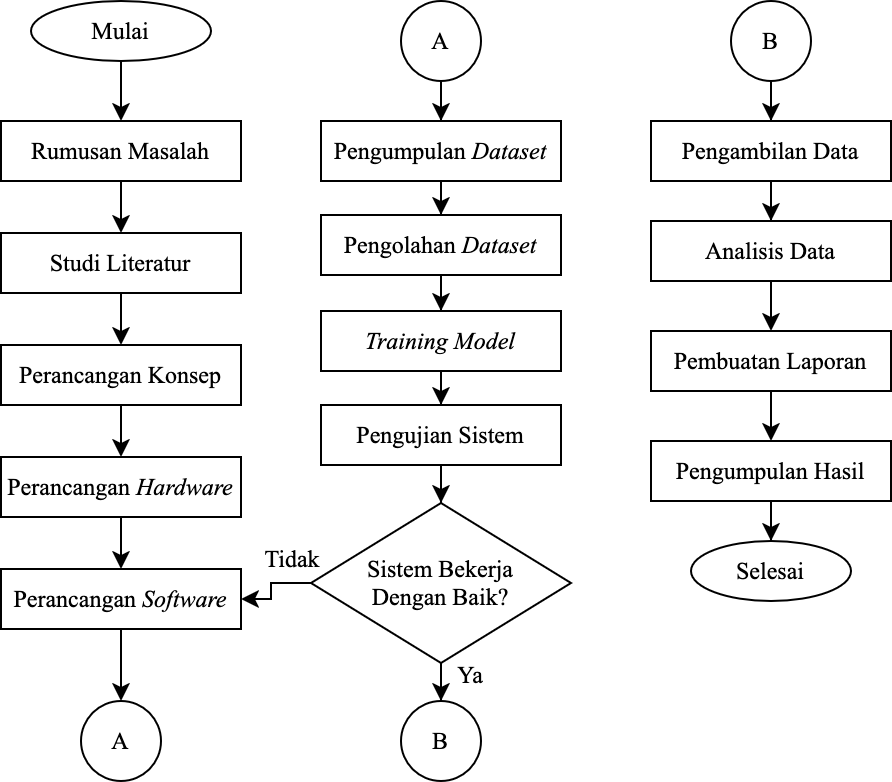
\includegraphics[width=0.9\textwidth]{images/flowchart_penelitian.png}
    \caption{Diagram Alir Penelitian}
    \label{fig:flowchart_penelitian}
\end{figure}

Penelitian ini dilaksanakan melalui serangkaian tahapan sistematis yang bertujuan untuk mengembangkan sistem pemodelan gerak tari tradisional Indonesia pada robot \textit{humanoid} berbasis estimasi pose 3D. Proses dimulai dengan perumusan masalah, yaitu mengidentifikasi tantangan utama dalam mengubah gerakan tari manusia menjadi representasi gerak yang dapat diimplementasikan pada robot. Setelah masalah dirumuskan, dilakukan studi literatur untuk memperoleh pemahaman yang mendalam mengenai teori dan teknologi yang mendasari, seperti metode \textit{pose estimation} (MeTRAbs, DeciWatch), pemrosesan dataset, dan pengendalian gerakan robot.
Penelitian ini dilakukan melalui serangkaian tahapan terstruktur yang bertujuan untuk menghasilkan sistem pemodelan gerak tari tradisional Indonesia pada robot \textit{humanoid} menggunakan metode estimasi pose. Alur penelitian diawali dengan identifikasi dan perumusan masalah, kemudian dilanjutkan dengan studi literatur untuk memperkuat dasar teori. Setelah itu dilakukan perancangan konsep dan perangkat lunak yang dibutuhkan, disusul oleh proses pengumpulan dan pengolahan data. 

Model dilatih menggunakan data yang telah disiapkan, kemudian diuji untuk menilai kinerjanya. Apabila hasil pengujian belum sesuai, dilakukan evaluasi dan perbaikan sistem. Jika sistem telah berfungsi dengan baik, proses dilanjutkan dengan pengambilan data hasil, analisis, penyusunan laporan, dan pengumpulan hasil akhir. 

\section{Metode Pengumpulan Data}

Pengumpulan data dilakukan untuk memperoleh informasi yang diperlukan dalam mendukung pelaksanaan penelitian, terutama terkait pengembangan dan pengujian sistem estimasi pose. Data yang digunakan dalam penelitian ini terdiri dari dua jenis utama, yaitu \textit{dataset} standar untuk pelatihan model dan data pengujian dari video tari tradisional Indonesia.

\subsection{\textit{Dataset} AIST++}

Penelitian ini menggunakan \textit{dataset} AIST++, yang merupakan salah satu \textit{benchmark dataset} standar untuk pelatihan dan evaluasi model estimasi pose manusia 3D, khususnya dalam konteks gerakan tari. \textit{AIST++} adalah \textit{dataset} yang dirancang untuk menangkap gerakan tari yang kompleks dan beragam, berisi lebih dari 10 juta frame video dengan anotasi pose 3D pada 60 fps~\shortcite{li2021ai}. \textit{Dataset} ini mencakup berbagai gaya tarian, seperti hip-hop, ballet, breakdance, jazz, dan gaya lainnya, yang memberikan keragaman gerakan tubuh secara spasial dan temporal, sehingga sangat cocok untuk melatih model yang fokus pada dinamika gerakan yang cepat dan bervariasi.

Dalam penelitian ini, digunakan dua jenis data dari \textit{dataset} AIST++ yakni hasil estimasi pose 3D dari video menggunakan model SPIN (\textit{SMPLify-X In the Loop}) dan data \textit{ground truth} pose 3D yang tersedia secara terbatas. Hal ini disebabkan oleh keterbatasan akses terhadap data video raw asli secara penuh, sehingga proses pelatihan model DeciWatch dilakukan menggunakan hasil prediksi SPIN sebagai data input dan data anotasi AIST++ sebagai target.

Data yang digunakan telah disusun dalam format .npz, yang berisi urutan pose 3D, parameter bentuk tubuh (shape), nama frame video, serta parameter kamera. Setiap file merepresentasikan satu sekuens gerakan dalam bentuk array dua dimensi, dengan jumlah frame yang bervariasi, rata-rata antara 300 hingga 600 frame per sekuens. Dataset ini dibagi menjadi dua bagian: data pelatihan (\textit{train}) sebanyak 7.292 sekuens dengan total 5.916.474 frame, dan data validasi (\textit{val}) sebanyak 3.840 sekuens dengan total 2.882.640 frame.

Penggunaan \textit{dataset} AIST++ dalam penelitian ini dimaksudkan untuk melatih dan mengevaluasi model DeciWatch agar mampu mengenali dan menyempurnakan estimasi pose manusia dalam konteks gerakan tari. Kompleksitas dan keragaman data AIST++ menjadikannya relevan untuk mengembangkan model yang nantinya diharapkan dapat diadaptasikan pada representasi gerakan tari tradisional Indonesia yang memiliki karakteristik gerak yang dinamis dan kompleks.


\begin{figure}[H]
    \centering
    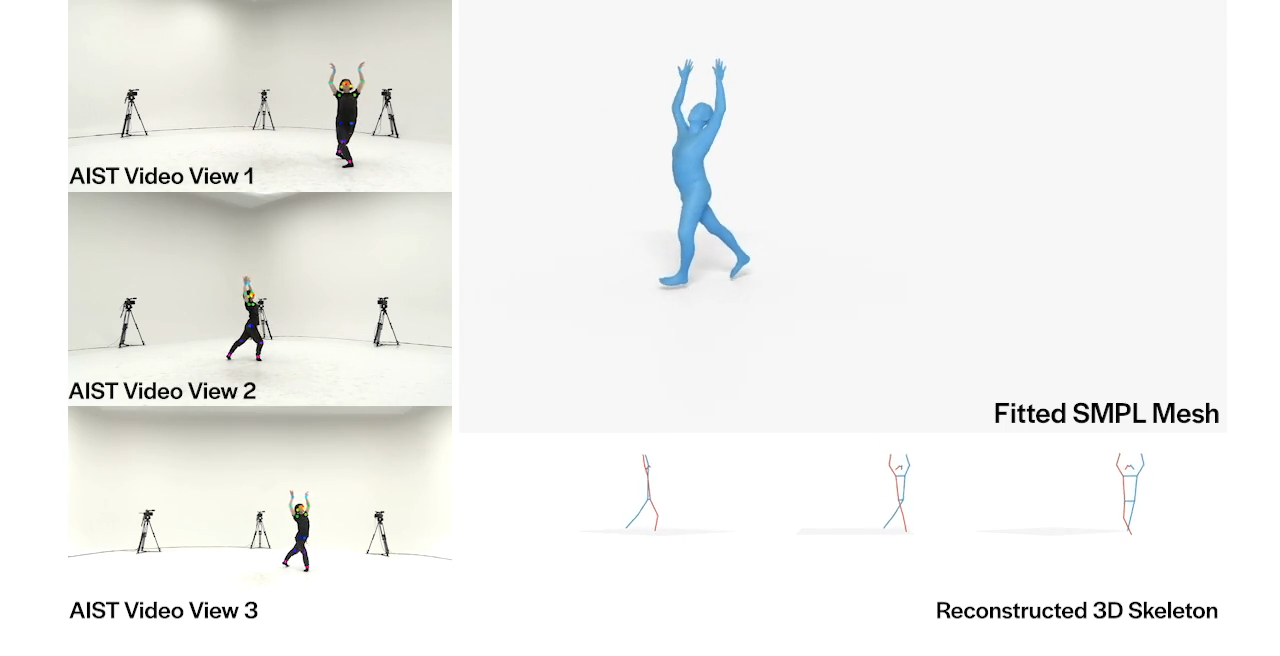
\includegraphics[width=0.7\textwidth]{images/aist.png}
    \captionsource{\textit{Dataset} AIST++}{\cite{li2021ai}}
    \label{fig:aist}
\end{figure}


\subsection{Data Video Tari Tradisional Indonesia}
Untuk pengujian model, data yang digunakan berasal dari video tari tradisional Indonesia yang diambil dari platform seperti YouTube. Video yang dipilih harus memenuhi beberapa kriteria, yaitu:
\begin{itemize}
    \item Menampilkan gerakan tari secara jelas dan berkelanjutan.
    \item Menggunakan teknik pengambilan gambar dengan kamera statis untuk meminimalkan gangguan visual.
    \item Memuat berbagai jenis tari tradisional Indonesia yang representatif.
\end{itemize}

Video-video ini kemudian diproses untuk menghasilkan \textit{keypoints} yang akan digunakan dalam evaluasi performa model estimasi pose. Sebagai contoh, gerakan tari seperti Denok Semarangan yang khas dan memiliki pola gerakan unik dapat menjadi bahan pengujian yang ideal untuk mengukur performa model.

\begin{figure}[H]
    \centering
    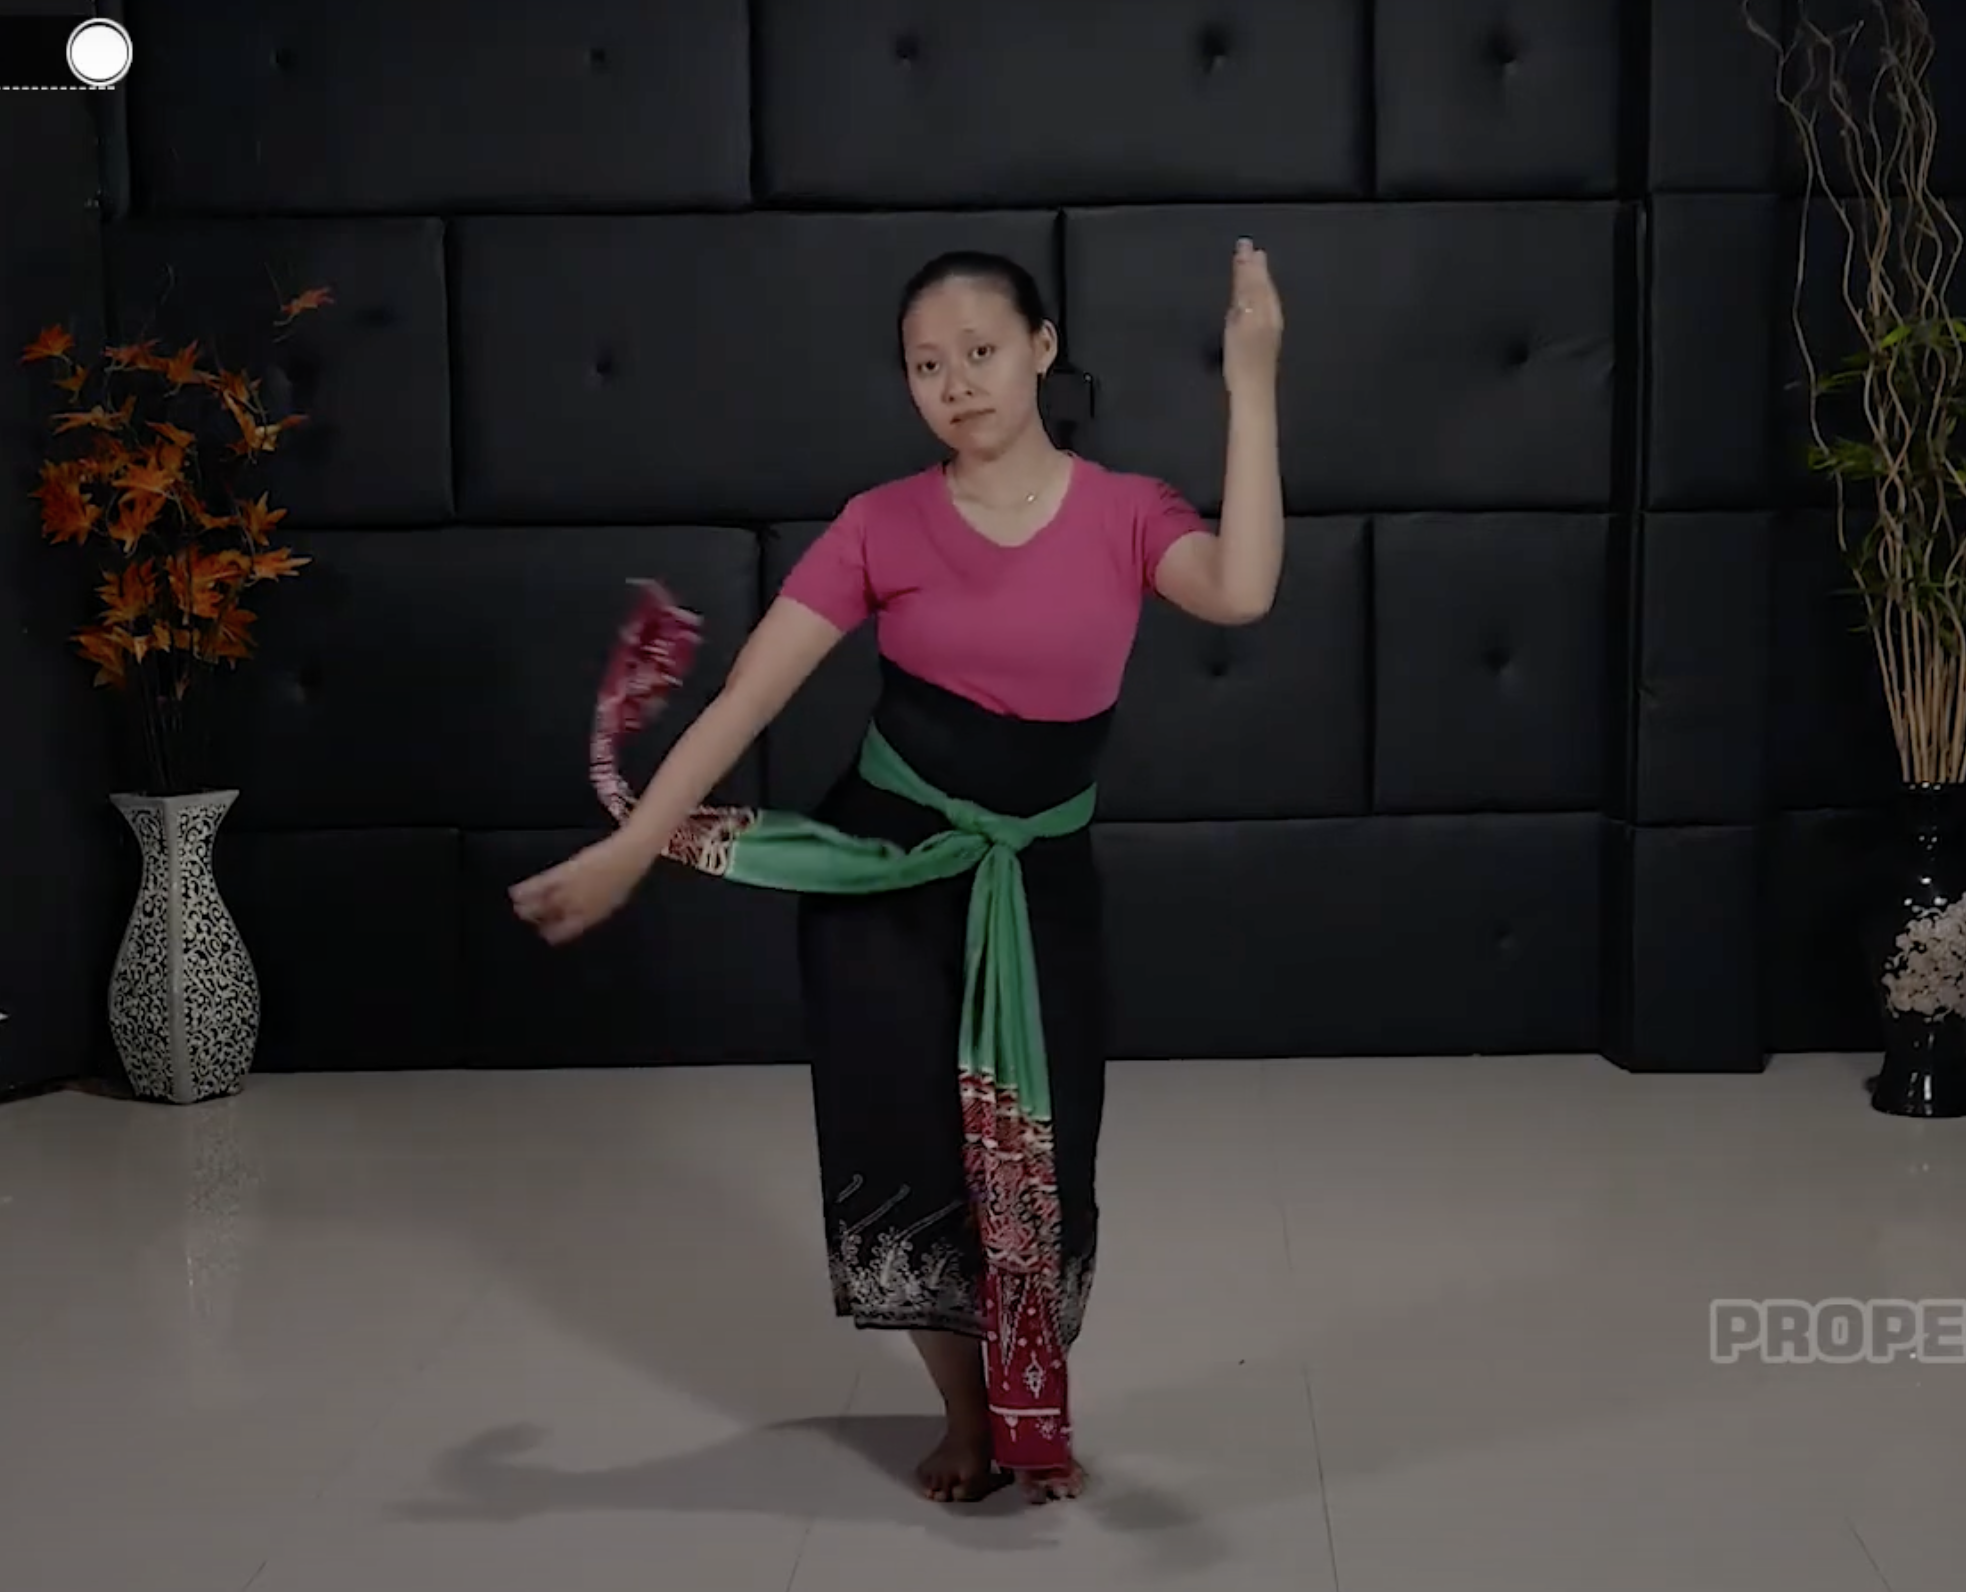
\includegraphics[width=0.5\textwidth]{images/dance_traditional.png}
    \captionsource{Tari Denok Semarangan}{YouTube}
    \label{fig:traditional_dance}
\end{figure}

\section{Teknik Pengolahan Data}

\begin{figure}[H]
    \centering
    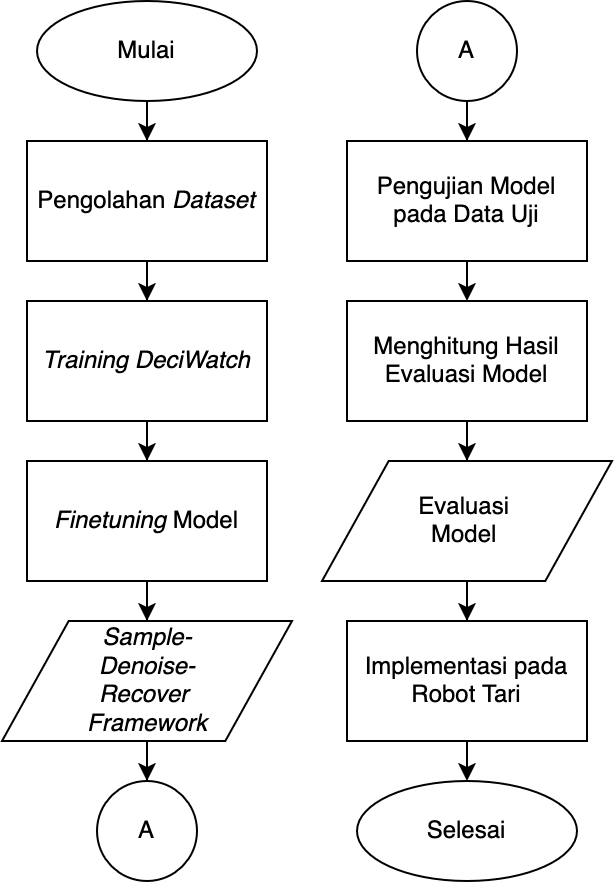
\includegraphics[width=0.5\textwidth]{images/flowchart_pengolahan.png}
    \caption{Diagram Alur Pengolahan Data}
    \label{fig:data_flowchart}
\end{figure}

\subsection{Pengolahan \textit{Dataset}}

Pada penelitian ini, \textit{dataset} yang digunakan berasal dari AIST++ Human Motion Dataset, yang sudah tersedia dalam bentuk data pose 3D yang siap digunakan tanpa perlu proses anotasi atau pengambilan data tambahan. Dataset ini telah diolah oleh pengembang DeciWatch dan dilengkapi dengan anotasi \textit{ground truth} serta hasil prediksi pose dari model SPIN. Struktur data AIST++ yang digunakan terdiri dari dua jenis data utama, yaitu:

\begin{itemize}
    \item \textit{Ground Truth Pose}: Berisi parameter koordinat 3D untuk 14 titik sendi tubuh.
    \item \textit{Predicted Pose (SPIN)}: Berisi hasil prediksi pose dari model SPIN yang berupa koordinat 3D titik sendi.
\end{itemize}

Adapun langkah-langkah pengolahan \textit{dataset} yang dilakukan dalam penelitian ini meliputi:

\begin{enumerate}
    \item {Pemilihan Data Latih dan Data Uji} \\
    Data dibagi menjadi dua bagian utama, yaitu data pelatihan (train) dan data pengujian (val). File {aist\_gt\_train.npz} dan {aist\_gt\_test.npz} digunakan untuk \textit{ground truth}, sedangkan {aist\_spin\_train.npz} dan {aist\_spin\_test.npz} digunakan untuk data prediksi SPIN.
    
    \item {Pemuatan dan Pemrosesan Struktur Data} \\
    Data dimuat menggunakan fungsi {numpy.load()} yang menghasilkan struktur dictionary berisi:
    \begin{itemize}
        \item {imgname}: Nama file dan indeks frame.
        \item {pose}: Parameter pose SMPL (72 dimensi).
        \item {trans}: Translasi gerakan 3D (3 dimensi).
        \item {scaling}: Faktor skala tubuh.
        \item {joints\_3d}: Koordinat 3D untuk 14 titik sendi utama.
    \end{itemize}
    
    \item {Pemetaan Keypoints} \\
    Data {joints\_3d} pada AIST++ memiliki urutan 14 titik sendi sesuai format: \textit{rankle, rknee, rhip, lhip, lknee, lankle, rwrist, relbow, rshoulder, lshoulder, lelbow, lwrist, neck, headtop}. Urutan ini identik dengan skema \textit{LSP-14} yang juga digunakan pada metode \textit{Metrabs}, sehingga kompatibel dengan standar pemetaan pose yang umum digunakan dalam literatur visi komputer. Pemetaan ini digunakan sebagai acuan dalam proses \textit{motion retargeting}, khususnya untuk menentukan titik-titik referensi pada perhitungan sudut sendi di robot humanoid.

    
    \item {Penyesuaian Input ke Model DeciWatch} \\
    Dataset ini kemudian digunakan sebagai input langsung ke model DeciWatch untuk proses prediksi pose berjangka waktu (temporal pose prediction). Karena DeciWatch membutuhkan input pose berurutan dalam bentuk sekuens, data pose diurutkan dan diproses dalam batch sesuai kebutuhan model.

\end{enumerate}

Proses ini tidak melibatkan anotasi manual karena seluruh data sudah tersedia dalam format yang sesuai untuk keperluan pelatihan dan pengujian model. Pengolahan dilakukan untuk memastikan data tersusun sesuai kebutuhan input pada sistem yang dikembangkan.


\subsection{\textit{Training} dan \textit{Fine-tuning} Model}
Setelah dataset hasil prediksi pose 3D oleh model Metrabs berhasil dikumpulkan dan diproses, langkah selanjutnya adalah melakukan pelatihan dan \textit{fine-tuning} model DeciWatch. Model ini bertujuan untuk meningkatkan akurasi estimasi pose secara temporal dengan memanfaatkan informasi antar-frame secara berurutan. 

Model DeciWatch dilatih menggunakan data input berupa pose 3D dari Metrabs sebagai \textit{frame-wise prediction}, kemudian disempurnakan melalui pembelajaran sekuensial untuk menghasilkan prediksi yang lebih halus dan akurat. Proses pelatihan dilakukan menggunakan \textit{framework} PyTorch dengan bantuan GPU yang mendukung CUDA dan cuDNN untuk mempercepat komputasi. Tahap \textit{fine-tuning} dilakukan dengan mengatur ulang parameter dan konfigurasi pelatihan agar model lebih sesuai dengan karakteristik data tari tradisional yang digunakan.


\subsection{Pengujian dan Evaluasi Model}

Model yang telah dilatih kemudian diuji menggunakan data uji yang berbeda dari data pelatihan untuk mengukur performanya. Evaluasi dilakukan dengan menghitung metrik \textit{Mean Per Joint Position Error} (MPJPE), yaitu rata-rata jarak Euclidean antara koordinat prediksi dan \textit{ground truth} dari setiap \textit{keypoint} dalam ruang 3D. Perhitungan MPJPE dilakukan sesuai dengan rumus yang telah dijelaskan pada Bab 2 pada persamaan (\ref{eq:mpjpe}). Nilai MPJPE yang lebih rendah menunjukkan akurasi prediksi yang lebih baik.

Proses evaluasi dilakukan dengan bantuan pustaka Python seperti NumPy untuk perhitungan matematis dan Matplotlib untuk analisis visualisasi hasil. Seluruh eksperimen dilakukan di lingkungan Jupyter Notebook atau Google Colab untuk mendukung fleksibilitas dalam pemrosesan dan pengujian model.




\subsection{Implementasi pada Robot Tari}
Setelah model dievaluasi, tahap berikutnya adalah implementasi pada robot humanoid ROBOTIS-OP3 untuk menguji kemampuan model dalam menghasilkan gerakan yang natural berdasarkan estimasi pose. Implementasi ini dilakukan dengan menggunakan bahasa pemrograman Python dan C++, serta memanfaatkan framework \textit{Robot Operating System} (ROS) untuk mengelola komunikasi antara perangkat keras dan perangkat lunak. Untuk menerjemahkan koordinat pose ke dalam pergerakan robot, digunakan konsep \textit{Inverse Kinematics} (IK) dengan dukungan pustaka Dynamixel SDK untuk mengontrol aktuator robot. Pengujian pergerakan robot juga dapat dilakukan di lingkungan simulasi menggunakan Gazebo dan Rviz sebelum diterapkan pada perangkat keras sebenarnya. 

% \section{Desain Sistem}
% \subsection{Diagram Blok Sistem}
% \begin{figure}[H]
%     \centering
%     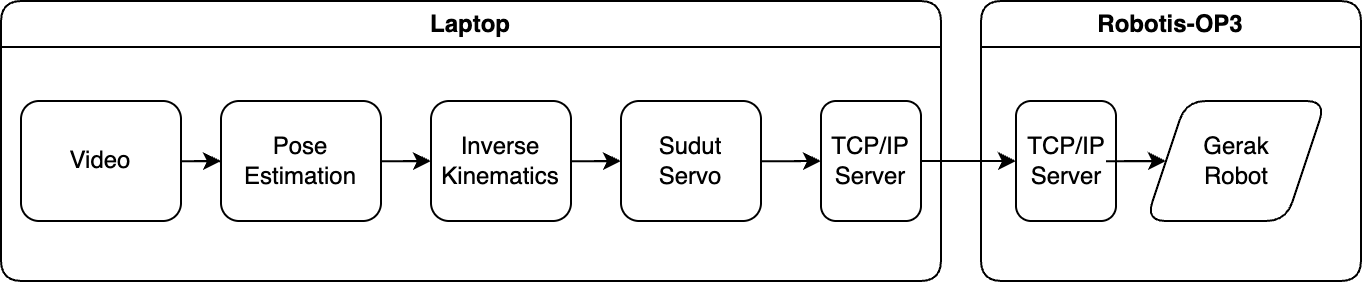
\includegraphics[width=0.8\textwidth]{images/sistem_diagram.png}
%     \caption{Diagram Sistem}
%     \label{fig:system_diagram}
% \end{figure}

% Seperti yang dapat dilihat pada Gambar \ref{fig:system_diagram}, input sistem berasal dari video yang memuat gerakan manusia. Data input ini kemudian diproses pada laptop menggunakan metode \textit{computer vision} dan \textit{deep learning} untuk melakukan estimasi pose tubuh manusia. Proses estimasi pose mendeteksi \textit{keypoints} tubuh, seperti kepala, tangan, dan kaki, yang kemudian dikonversi menjadi koordinat spasial. Selanjutnya, data pose ini diproses menggunakan metode \textit{inverse kinematics} untuk menghitung sudut-sudut sendi (\textit{servo angles}) yang sesuai. Data hasil perhitungan ini dikirimkan ke robot ROBOTIS-OP3 melalui protokol komunikasi TCP/IP bawaan ROS. Setelah diterima oleh robot, data sudut servo digunakan untuk menggerakkan robot, sehingga robot dapat mereplikasi gerakan yang ditampilkan dalam input. Output dari sistem adalah gerakan robot humanoid yang sesuai dengan data pose dari input video.

% \subsection{Flowchart Sistem}
% \vspace{1 em}
% \begin{figure}[H]
%     \centering
%     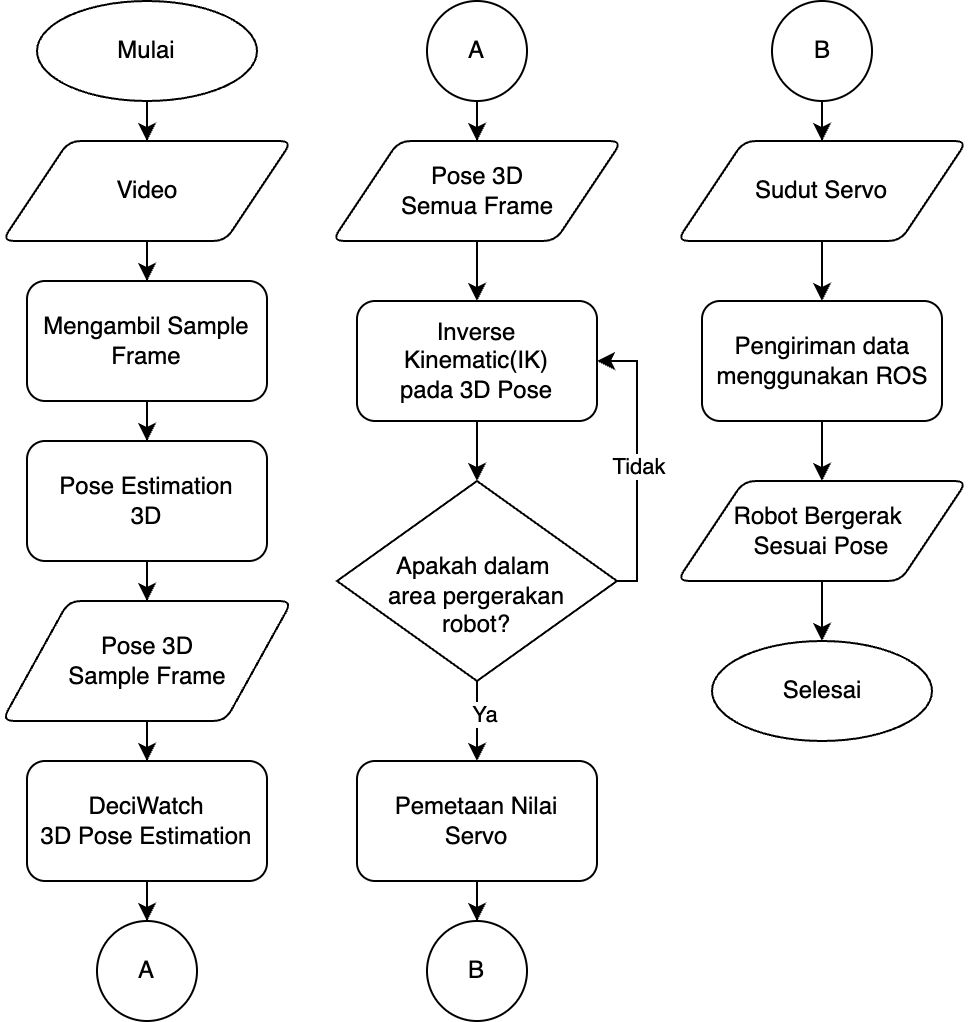
\includegraphics[width=0.7\textwidth]{images/flowchart.png}
%     \caption{Flowchart System}
%     \label{fig:system_flowchart}
% \end{figure}


% Flowchart pada Gambar \ref{fig:system_flowchart} menggambarkan alur proses estimasi pose 3D menggunakan metode DeciWatch serta implementasinya pada robot humanoid. Proses dimulai dengan input berupa video yang menjadi sumber data utama. Dari video ini, sampel frame diambil untuk mengurangi beban komputasi sekaligus memastikan kualitas data yang representatif untuk analisis pose.

% Setelah frame sampel diambil, pendapatan pose 3D awal dilakukan menggunakan model SPIN (\textit{SMPLify-X in the Loop}), yang merupakan salah satu metode estimasi pose 3D yang andal. SPIN menghasilkan pose 3D untuk setiap frame sampel, mencakup koordinat 3D dari titik-titik penting tubuh manusia. Data pose 3D awal ini kemudian diproses lebih lanjut menggunakan metode DeciWatch. DeciWatch memanfaatkan pendekatan \textit{sample-denoise-recover} untuk memperbaiki pose 3D dari frame yang telah dipilih, menghasilkan pose 3D yang lebih halus dan akurat dengan efisiensi komputasi yang tinggi.

% Pada bagian A, data pose 3D dari semua frame yang telah diproses menggunakan DeciWatch dilanjutkan dengan algoritma \textit{Inverse Kinematics} (IK). Algoritma IK bertugas untuk menghitung parameter gerakan robot berdasarkan pose 3D, serta memastikan apakah pose tersebut berada dalam area pergerakan robot. Jika pose tidak sesuai, proses kembali ke langkah IK untuk dilakukan penyesuaian. Namun, jika pose berada dalam area yang sesuai, data tersebut diteruskan ke proses pemetaan nilai servo.

% Bagian B mencakup pemetaan sudut servo berdasarkan data yang dihasilkan dari algoritma IK. Sudut servo yang telah dihitung kemudian dikirimkan ke robot menggunakan \textit{Robot Operating System} (ROS). Dengan ROS, data dikirimkan secara real-time untuk mengontrol pergerakan robot humanoid. Akhirnya, robot bergerak sesuai dengan pose yang telah dihitung, menghasilkan gerakan yang natural dan sesuai dengan data pose 3D awal.

% Flowchart ini mengintegrasikan berbagai komponen utama, seperti estimasi pose awal menggunakan SPIN, perbaikan pose menggunakan DeciWatch, algoritma IK, pemetaan servo, dan implementasi kontrol gerakan melalui ROS. Integrasi ini menghasilkan sistem yang efisien dan akurat untuk mengontrol gerakan robot berdasarkan data pose 3D.

\section{Uji Coba Sistem}

Uji coba sistem dilakukan untuk mengevaluasi keandalan dan kesesuaian fungsional sistem dalam mereplikasi gerakan manusia menggunakan robot humanoid ROBOTIS-OP3. Proses uji coba mencakup dua jenis pengujian utama, yaitu pengujian fungsional berupa \textit{black-box testing} dan pengujian performa dari model estimasi pose serta implementasi gerakan pada robot.

Secara umum, uji coba sistem difokuskan pada dua aspek utama berikut:

\begin{itemize}
    \item {Pengujian Fungsional Sistem (\textit{Black-Box Testing})}, yaitu pengujian terhadap alur kerja sistem secara keseluruhan, mulai dari input data gerak, pemrosesan melalui antarmuka berbasis \textit{website}, hingga eksekusi gerakan pada robot. Pengujian ini memastikan bahwa seluruh komponen sistem dapat berfungsi dengan baik tanpa melihat detail proses di dalamnya.
    
    \item {Pengujian Performa Estimasi dan Reproduksi Gerakan}, meliputi:
    \begin{itemize}
        \item \textit{Akurasi prediksi pose temporal} dari model DeciWatch, dengan evaluasi menggunakan metrik \textit{Mean Per Joint Position Error (MPJPE)} seperti pada persamaan (\ref{eq:mpjpe}).
        \item \textit{Kesesuaian hasil motion retargeting} pada robot ROBOTIS-OP3, yaitu evaluasi kualitas reproduksi gerakan robot terhadap urutan pose hasil prediksi serta kelancaran eksekusi pada saat proses \textit{playback}.
    \end{itemize}
\end{itemize}

Evaluasi ini dilakukan untuk memastikan sistem bekerja secara fungsional dan juga memiliki tingkat akurasi serta performa gerakan yang sesuai dengan kebutuhan pemodelan gerak tari tradisional Indonesia.


